\documentclass[11pt,oneside,a4paper]{article}
\usepackage[utf8]{inputenc}
\date{}
\usepackage[linesnumbered,ruled,vlined]{algorithm2e}
\SetKwInput{KwInput}{Input}                % Set the Input
\SetKwInput{KwOutput}{Output}              % set the Output<z
\usepackage{blindtext}
\usepackage{changepage}

\usepackage{amsmath}
\usepackage{color}
\usepackage{tcolorbox}
\usepackage{sectsty}
\usepackage{stmaryrd}
\usepackage{gensymb}
\usepackage{wasysym}
\usepackage{amsfonts}
\usepackage{xcolor}
\usepackage{graphicx}
\usepackage{stmaryrd}
\usepackage{mathtools}
\usepackage{amsthm}
\usepackage{caption}
\usepackage{subcaption}
\usepackage[margin=1.2in]{geometry}
%__________WIDE HAT_________
\usepackage{scalerel,stackengine}
\stackMath
\newcommand\reallywidehat[1]{%
\savestack{\tmpbox}{\stretchto{%
  \scaleto{%
    \scalerel*[\widthof{\ensuremath{#1}}]{\kern-.6pt\bigwedge\kern-.6pt}%
    {\rule[-\textheight/2]{1ex}{\textheight}}%WIDTH-LIMITED BIG WEDGE
  }{\textheight}%
}{0.5ex}}%
\stackon[1pt]{#1}{\tmpbox}%
}
\parskip 1ex
%______________________________
\usepackage{hyperref}
\hypersetup{
    colorlinks=true,
    urlcolor=blue
}
\setlength{\parindent}{0in}
\theoremstyle{definition}
\newtheorem{definition}{Definition}[section]

\theoremstyle{remark}
\newtheorem*{remark}{Remark}
\usepackage{amsmath}
\usepackage[T1]{fontenc}
\usepackage{float}
\usepackage[british,UKenglish,swedish,USenglish,english,american]{babel}
\usepackage[T1]{fontenc}
\usepackage{fancyhdr}
\usepackage{natbib}
%\pagestyle{fancy}
\begin{document}
\renewcommand{\bibname}{References}
\hypersetup{citecolor=black}
\begin{titlepage}\centering
\vspace*{\fill}
\Huge Assignment 2\\
\vspace*{10mm}
\large Includes methods of Directed Graphical Models, Dynamic programming, Variational Inference and Expectation Maximisation \\
\vspace*{\fill}
\large \textsc{DD2434 Advanced Machine Learning} \\
\textsc{Filip Bergentoft, bergento@kth.se} \\
\end{titlepage}

\newpage

%qqq: Add figures to problem 1
\section*{Problem 1}
Let $\theta = (\theta^r, \theta^e, \theta^a, \psi)$ and $X_{nlm} = 1$ if reader $n$ has clicked on advertisement $m$ in edition $l$, $X_{nlm} = 0$, otherwise.


The ECLL is given by

\begin{align*}
  ECLL = \sum_{nlm} \mathbb{E}_p(Z|)
\end{align*}










Given that we can observe both $Z$ and $X$ we get the following likelihood

\begin{align*}
  L(\theta; D) & = \prod_{n,l,m}p(X_{nlm}, Z_n^r, Z_l^r, Z_m^a | \psi) \\
  & = \prod_{nlm} \prod_{cdf} (\theta_c^r)^{ I(Z_n^r = c)} (\theta_d^e)^{ I(Z_l^e = d)}
  (\theta_f^a)^{ I(Z_m^a = f)} p(X_{nlm} |\psi_{cdf})^{I((Z_n^r, Z_l^r, Z_m^a) = (c,d,f)}
\end{align*}

Can now look at the log-likelihood

\begin{align*}
    l(\theta; D) & = \sum_{nlm}\sum_{cdf} I(Z_n^r = c) ln(\theta_c^r) + I(Z_l^e = d) ln(\theta_d^e)
    + I(Z_m^a = f) ln(\theta_f^a) \\
    & + I((Z_n^r, Z_l^r, Z_m^a) = (c,d,f)) ln(p(X_{nlm} |\psi_{cdf}))
\end{align*}

Now let

\begin{align*}
  & A = \sum_{cdf}\sum_{nlm} I(Z_n^r = c) ln(\theta_c^r) + I(Z_l^e = d) ln(\theta_d^e)
  + I(Z_m^a = f) ln(\theta_f^a) \\
  & B = \sum_{nlm}\sum_{cdf} I((Z_n^r, Z_l^r, Z_m^a) = (c,d,f)) ln(p(X_{nlm} |\psi_{cdf}))
\end{align*}

Can then rewrite $A$ in the following manner

\begin{align*}
  A = \sum_{cdf} LM N_c^r ln(\theta_c^r) + NM N_d^e ln(\theta_d^e) + NL ln(\theta_f^a)
\end{align*}

Where each term can be maximised independently using known techniques from lectures yielding

\begin{align*}
  & \theta_c^r = \frac{N^r_c}{N} \\
  & \theta_d^e = \frac{N^e_d}{L} \\
  & \theta_c^r = \frac{N^a_f}{M}
\end{align*}


%qqq:Need to read through - make sure it is understandable
\section*{2.2 Likelihood of a Tree Graphical Model}


\begin{tcolorbox}
\textbf{Question 2.2.7:}
Implement a dynamic programming algorithm that, for a given $T, \Theta \text{ and } \beta$ computes $p(\beta | T, \Theta)$
\end{tcolorbox}

$T$ is a binary tree with a vertex set $V(T)$ and a leaf set $L(T)$. For each vertex $v \in V(T)$ there is an associated random variable $X_v \in [K]$ with a corresponding CPD $\theta_v = p(X_v|x_{pa(v)})$ which is a categorical distribution. $\beta$ is defined as the set of values of all leafs in $T$ such that $\beta = \{x_l \, : \, l \in L(T)$.

In order to compute $p(\beta | T, \Theta)$ we need to find an expression that can be used for dynamic programming, I.E. splitting up the full problem into smaller subproblems. By looking at the definition of $s$ in equation (\ref{def_s})

\begin{equation}
  s(u,i) = p(X_{Observed \, \cap \, \downarrow u}| X_u = i)
  \label{def_s}
\end{equation}

and letting the root node of the tree being denoted by $r$, one can use that if $u$ is chosen as the root $r$ we get the following expression

\begin{align*}
  s(r,i) = p(X_{Observed \, \cap \, \downarrow r}| X_r = i) = \bigg\{ X_{Observed \, \cap \, \downarrow r} = \beta \bigg\} = p(\beta | X_r = i, T, \Theta)
\end{align*}

We can then marginalise this using Bayes' theorem in the following manner

\begin{align}
  p(\beta | T, \Theta) & = \sum_i p(\beta, X_r = i| T, \Theta) = \sum_i p(\beta | X_r = i, T, \Theta)p(X_r = i) \\
  & = \sum_i s(r,i)p(X_r = i)
  \label{sol_eq}
\end{align}

Using that $T$ is a binary tree and thus if $v, w$ are children to a node $u$ then

\begin{align}
  s(u,i) & = p(X_{Observed \, \cap \, \downarrow u}| X_u = i)\nonumber \\
  & = p(X_{Observed \, \cap \, \downarrow v}| X_v = i)
  p(X_{Observed \, \cap \, \downarrow w}| X_w = i) \nonumber\\
  & = \bigg( \sum_j s(v,j)p(X_v = j| x_u = i) \bigg )\bigg( \sum_j s(w,j)p(X_w = j| x_w = i) \bigg )
  \label{traverse_eq}
\end{align}

A special case is when the node $u$ is a leaf node, then the following holds

\begin{align}
  s(u,i) = \begin{cases} 1, & X_u = i \\ 0, & otherwise\end{cases}
  \label{eq_3}
\end{align}


Equation (\ref{sol_eq}) can then be computed using dynamic programming by starting at the leaf nodes using equation (\ref{eq_3}) and then traversing up the nodes in the tree to the root using equation (\ref{traverse_eq}) one level at a time and storing the achieved probabilities $s$ along the way.
\\

\begin{tcolorbox}
\textbf{Question 2.2.8:}
Apply your algorithm to the graphical model and data provided separately
\end{tcolorbox}

The following likelihoods were achieved when applying my implementation of the dynamic programming algorithm on the given trees.


\begin{center}
    \begin{tabular}{ | c | c | c |  c | c | c |}
    \hline
    Tree sample: & $0$ & $1$ & $2$ & $3$ & $4$ \\ \hline
    Small tree & $0.016$ & $0.015$ & $0.011$ & $0.007$ & $0.041$ \\ \hline
    Medium tree & $4.336 \cdot 10^{-18}$ & $3.094 \cdot 10^{-20}$ & $1.050 \cdot 10^{-16}$ & $6.585 \cdot 10^{-16}$ & $1.488 \cdot 10^{-18}$ \\ \hline
    Large tree & $3.288 \cdot 10^{-69}$ & $1.109 \cdot 10^{-66}$ & $2.522 \cdot 10^{-68}$ & $1.242 \cdot 10^{-66}$ & $3.535 \cdot 10^{-69}$ \\ \hline
    \end{tabular}
\end{center}


\section*{3.3 Complicated likelihood for leaky units on a tree}
\begin{tcolorbox}
  \textbf{Problem formulation:} Consider the following model. A binary tree $T$ has random variables associated with its vertices. A vertex $u$ has an observable variable $X_{u}$ and a latent class variable $Z_{u} .$ Each class $c \in[C]$ has a normal distribution $N\left(\mu_{k}, \sigma^{2}\right) .$ If the three neighbors of $u$ are $v_{1}, v_{2},$ and $v_{3},$ then
  $$
  p\left(X_{u} \mid Z_{u}=c, Z_{v_{1}}=c_{1}, Z_{v_{2}}=c_{2}, Z_{v_{2}}=c_{2}\right) \sim N\left(X_{u} \mid(1-\alpha) \mu_{c}+\sum_{i \in[3]} \frac{1}{3} \alpha \mu_{c_{i}}, \sigma^{2}\right)
  $$
  The class variables are iid, each follows the categorical distribution $\pi .$ Provide a linear time algorithm that computes $P(X \mid T, M, \sigma, \alpha, \pi)$ when given a tree $T$ (with vertices $V(T))$, observable variables for its vertices $X=\left\{X_{v}: v \in V(T)\right\},$ and parameters $M=\left\{\mu_{c}: c \in[C]\right\}, \sigma, \alpha .$
\end{tcolorbox}
We are interested in finding the likelihood of our observations $X$ by marginalising the following
\begin{equation}
  p(X) = \sum_Z p(X,Z)
\end{equation}
where $\sum_Z$ denotes the sum over all latent variables. We will show how this problem can be continuously split up into smaller and smaller subproblems using the structure of the binary tree until the leaves are reached. This will result in a linear algorithm for computing the requested likelihood $P(X \mid T, M, \sigma, \alpha, \pi)$ which we will from now on denote as $p(X)$ for the sake of brevity.

\subsection*{Starting at the root}
We will start by showing how one can split the problem into two subproblems when starting at the root.

Let $u$ denote the root and $u_1, u_2$ denote its children as in figure \ref{root_case}.
\begin{figure}[H]
\begin{center}
  \scalebox{0.7}{
  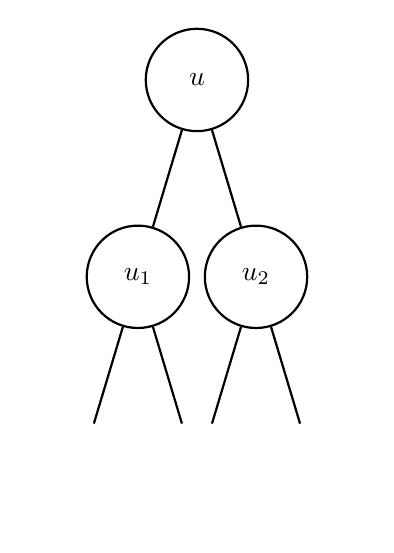
\begin{tikzpicture}[thick, minimum size=1.3cm, level distance=2.5cm]
    \node[circle,draw]{$u$}
        child { node[circle,draw]{$u_1$}
            child { node[circle]{}}
            child { node[circle]{}}
        }
        child { node[circle,draw]{$u_2$}
            child { node[circle]{}}
            child { node[circle]{}}
        };
  \end{tikzpicture}
  }
\end{center}
\caption{Binary tree starting at root r, branches below $u_1, u_2$ denotes subtrees}
\label{root_case}
\end{figure}

We begin by using that the root $u$ is independent of its children given $Z_u, Z_{u_1}, Z_{u_2}$ which leads to the following factorisation.
\begin{align}
  p(X) & = \sum_Z p(X,Z) = \sum_Z p(X_u, X_{u_1}, X_{u_2}, X_{u_1\downarrow}, X_{u_2\downarrow}, Z) \nonumber \\
  & = \sum_Z p(X_u, X_{u_1}, X_{u_2}, X_{u_1\downarrow}, X_{u_2\downarrow}, Z_{u_1\downarrow}, Z_{u_2\downarrow}| Z_u, Z_{u_1}, Z_{u_2})p(Z_u, Z_{u_1}, Z_{u_2}) \nonumber\\
  & = \sum_Z p(X_u|Z_{u_1}, Z_{u_2}, Z_u) p(Z_{u_1}, Z_{u_2}, Z_u)
  p(X_{u_1}, X_{u_1 \downarrow}, Z_{u_1 \downarrow}|Z_{u_1}, Z_u)
  p(X_{u_2}, X_{u_2 \downarrow}, Z_{u_2 \downarrow}|Z_{u_2}, Z_u) \nonumber\\
\end{align}
We can now let the sums over $Z_{u_1 \downarrow}$ and $Z_{u_2 \downarrow}$ move in which yields that
\begin{align}
  p(X) & = \sum_{Z_u, Z_{u_1}, Z_{u_2}}\bigg[p(X_u|Z_{u_1}, Z_{u_2}, Z_u) p(Z_{u_1}, Z_{u_2}, Z_u) \nonumber\\
  & \qquad\qquad\quad \Big(\sum_{Z_{u_1 \downarrow}} p(X_{u_1}, X_{u_1 \downarrow}, Z_{u_1 \downarrow}|Z_{u_1}, Z_u) \Big)\Big(\sum_{Z_{u_2 \downarrow}} p(X_{u_2}, X_{u_2 \downarrow}, Z_{u_2 \downarrow}|Z_{u_2}, Z_u) \Big)\bigg] \nonumber \\
\end{align}
Using that the latent variables $Z$ are independent given $\pi$ and substituting for the available densities yields
\begin{align}
  p(X) & = \sum_{Z_u, Z_{u_1}, Z_{u_2}}\bigg[\mathcal{N}\Big(X_u|(1-\alpha)\mu_{Z_u} +\frac{\alpha}{2}(\mu_{Z_{u_1}}+\mu_{Z_{u_2}}), \sigma^2 \Big) \pi(Z_u) \pi(Z_{u_1}) \pi(Z_{u_2})\\
  & \qquad\quad
  \Big(\underbrace{\sum_{Z_{u_1 \downarrow}} p(X_{u_1}, X_{u_1 \downarrow}, Z_{u_1 \downarrow}|Z_{u_1}, Z_u)}_\text{$p_{Z_{u_1 \downarrow}}$} \Big)
  \Big(\underbrace{\sum_{Z_{u_2 \downarrow}} p(X_{u_2}, X_{u_2 \downarrow}, Z_{u_2 \downarrow}|Z_{u_2}, Z_u)}_\text{$p_{Z_{u_2 \downarrow}}$} \Big) \bigg]
\end{align}
Where $p_{Z_{u_1 \downarrow}}$ and $p_{Z_{u_2 \downarrow}}$ denotes two independent subproblems with respect to the sets of latent variables $Z_{u_1 \downarrow}$ and $Z_{u_2 \downarrow}$

\subsection*{Starting at a node within the tree}
Now we will show how we can continue to divide each subproblem $p_{Z_{u_1 \downarrow}}$ and $p_{Z_{u_2 \downarrow}}$ defined above until the leaves are reached. We will now let $u_{1}$ and $u_{2}$ be the children of node $u$ and we will treat the problem shown in figure \ref{within_tree}


\begin{figure}[H]
\begin{center}
  \scalebox{0.7}{
  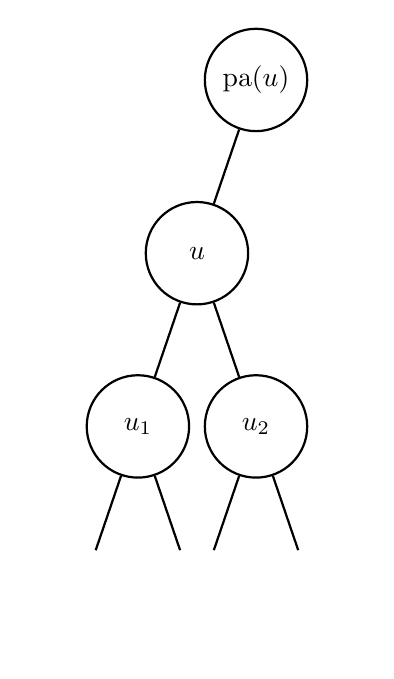
\begin{tikzpicture}[thick, minimum size=1.3cm, level distance=2.2cm]
    \node[circle,draw]{pa$(u)$}
        child { node[circle,draw]{$u$}
            child { node[circle,draw]{$u_1$}
                child { node[circle]{} }
                child { node[circle]{} }
                }
            child { node[circle,draw]{$u_2$}
                child { node[circle]{} }
                child { node[circle]{} }
                }
        }
        child [ missing ];
  \end{tikzpicture}
  }
\end{center}
  \caption{Binary tree starting at parent of $u$, branches below $u_1, u_2$ denotes subtrees}
  \label{within_tree}
\end{figure}

Let $p_{Z_{u \downarrow}} = \sum_{Z_{u \downarrow}} p(X_u, X_{u \downarrow}, Z_{u \downarrow}|Z_u, Z_{\text{pa}(u)})$, then

\begin{align}
  p_{Z_{u \downarrow}} & = \sum_{Z_{u \downarrow}} p(X_u, X_{u_1}, X_{u_2}, X_{u_1 \downarrow}, X_{u_2 \downarrow}, Z_{u_1 \downarrow}, Z_{u_2 \downarrow}|Z_u, Z_{\text{pa}(u)}, Z_{u_1}, Z_{u_2})p(Z_{u_1}) p(Z_{u_1\downarrow}) \nonumber \\
  & = \sum_{Z_{u \downarrow}} p(X_u|Z_u, Z_{\text{pa}(u)}, Z_{u_1}, Z_{u_2}) p(Z_{u_1})p(Z_{u_2})p(X_{u_1}, X_{u_1\downarrow}, Z_{u_1\downarrow}|Z_{u_1}, Z_u) p(X_{u_2}, X_{u_2\downarrow}, Z_{u_2\downarrow}|Z_{u_2}, Z_u) \nonumber\\
  & = \sum_{Z_{u \downarrow}} \bigg[ p(X_u|Z_u, Z_{\text{pa}(u)}, Z_{u_1}, Z_{u_2})p(Z_{u_1})p(Z_{u_2}) \nonumber\\
  & \qquad\qquad p(X_{u_1}, X_{u_1\downarrow}, Z_{u_1\downarrow}|Z_{u_1}, Z_u) p(X_{u_2}, X_{u_2\downarrow}, Z_{u_2\downarrow}|Z_{u_2}, Z_u) \bigg] \nonumber\\
  & = \sum_{Z_{u_1}, Z_{u_2}} \bigg[ p(X_u|Z_u, Z_{\text{pa}(u)}, Z_{u_1}, Z_{u_2})p(Z_{u_1})p(Z_{u_2}) \nonumber\\
  & \qquad\qquad
  \Big( \sum_{Z_{u_1\downarrow}} p(X_{u_1}, X_{u_1\downarrow}, Z_{u_1\downarrow}|Z_{u_1}, Z_u) \Big)
  \Big( \sum_{Z_{u_2\downarrow}} p(X_{u_2}, X_{u_2\downarrow}, Z_{u_2\downarrow}|Z_{u_2}, Z_u)\Big) \bigg] \nonumber\\
  & = \sum_{Z_{u_1}, Z_{u_2}} \bigg[ p(X_u|Z_u, Z_{\text{pa}(u)}, Z_{u_1}, Z_{u_2})p(Z_{u_1})p(Z_{u_2}) \Big(p_{Z_{u_1\downarrow}}\Big) \Big( p_{Z_{u_2\downarrow}}\Big)\bigg] \nonumber \\
  & = \sum_{Z_{u_1}, Z_{u_2}} \bigg[ \mathcal{N}\Big(X_u|(1-\alpha)\mu_{Z_u} +\frac{\alpha}{3}(\mu_{Z_{u_1}}+\mu_{Z_{u_2}}+\mu_{Z_{\text{pa}(u)}}), \sigma^2 \Big) \cdot \nonumber\\
  & \qquad\qquad\qquad  \cdot \pi(Z_{u_1}) \pi(Z_{u_2}) \Big(p_{Z_{u_1\downarrow}}\Big) \Big( p_{Z_{u_2\downarrow}}\Big)\bigg]\nonumber
\end{align}

On a more compact form we have thus shown that

\begin{align}
  p_{Z_{u \downarrow}} & = \sum_{Z_{u \downarrow}} p(X_u, X_{u \downarrow}, Z_{u \downarrow}|Z_u, Z_{\text{pa}(u)}) \\
  & = \sum_{Z_{u_1}, Z_{u_2}} \bigg[ \mathcal{N}\Big(X_u|(1-\alpha)\mu_{Z_u} +\frac{\alpha}{3}(\mu_{Z_{u_1}}+\mu_{Z_{u_2}}+\mu_{Z_{\text{pa}(u)}}), \sigma^2 \Big) \cdot \label{rec1}\\
  & \qquad\qquad\qquad  \cdot \pi(Z_{u_1}) \pi(Z_{u_2}) \Big(p_{Z_{u_1\downarrow}}\Big) \Big( p_{Z_{u_2\downarrow}}\Big)\bigg] \label{rec2}
\end{align}
Which shows the recursion.


We have thus ended up with two new subproblems $p_{Z_{u_1\downarrow}}$ and $p_{Z_{u_2\downarrow}}$ from $p_{Z_{u \downarrow}}$ which can be divided into subproblems continuously until the leaves are reached.
\\

It is important to note that $p_{Z_{u_1\downarrow}}$ is independent of $Z_{u_2}$ and similarly $p_{Z_{u_2\downarrow}}$ is independent of $Z_{u_1}$. It is thus only necessary to compute $p_{Z_{u_1\downarrow}}$ when summing over $Z_{u_1}$. When summing over $Z_{u_2}$ the value for $p_{Z_{u_1\downarrow}}$ can be computed once, stored and then be reused. Applying this for all subproblems results in a linear algorithm for computing $p(X)$.


\subsection*{Starting at a leaf}
When equation \eqref{rec1} $+$ \eqref{rec2} has been used recursively until the leaves are reached we need to show that the DP-algorithm can be started there. Let $u_1$ denote a \textit{leaf node}, it thus has no children which implies that $Z_{u_1 \downarrow} = \emptyset$. Using previous definition of $p_{Z_{u \downarrow}}$ yields

 \begin{align}
   p_{Z_{u_1 \downarrow}} & = \sum_{Z_{u_1 \downarrow}} p(X_{u_1}, X_{u_1 \downarrow}, Z_{u_1 \downarrow}|Z_{u_1}, Z_{\text{pa}(u_1)}) \nonumber\\
   & = p(X_{u_1}|Z_{u_1}, Z_{\text{pa}(u_1)}) \nonumber\\
   & = \mathcal{N}\Big(X_{u_1} | (1-\alpha)\mu_{Z_{u_1}} + \alpha \mu_{Z_{\text{pa}(u_1)}}, \sigma^2 \Big)
 \end{align}


\section*{2.4 Mixture of trees with observable variables}

\begin{tcolorbox}
\textbf{Question 2.4.12:}
Implement this EM algorithm.
\end{tcolorbox}
The EM algorithm with sieving was was implemented in the following manner using the given Tree package.

\begin{algorithm}[H]
\SetAlgoLined
\KwInput{Data samples}
\KwOutput{Tree mixture}

  Compute a distance matrix of the data: $D \gets \text{weighted\_distance} (Y) $

  Compute a similarity matrix from $D$: $S \gets \text{similarity\_matrix} (D) $

  Compute Eigen-decomposition of $S$: $[D,Q] \gets \text{Eig}(S)$

  Order $D$ in descending order of eigenvalues magnitude and $Q$ correspondingly

  Ensure elements of $D$ and $Q$ are real

  Compute embedding: $X \gets I_{2\times 101}D Q^T$

  \caption{EM algorithm}
\end{algorithm}

\begin{tcolorbox}
\textbf{Question 2.4.13:}
Apply your algorithm to the provided data and show how well you reconstruct the mixtures. First, compare the real and inferred trees with the unweighted Robinson-Foulds (aka symmetric difference) metric. Do the trees have similar structure? Then, compare the likelihoods of real and inferred mixtures.
\end{tcolorbox}

\begin{tcolorbox}
\textbf{Question 2.4.14:}
Simulate new tree mixtures with different number of nodes, samples and clusters. Try to find some interesting cases. Analyse your results as in the previous question.
\end{tcolorbox}


\end{document}
